Having covered the importance of LLM optimization and the technical architecture of transformers in previous chapters, we now turn to the practical challenge of model compression.

This chapter begins with preliminary experiments on layer manipulation that revealed crucial insights about architectural redundancy in transformer models and shaped the main compression strategy. It then presents what is possibly the heart of this research: a multi-stage pipeline that combines several optimization techniques in a structured sequence. Each stage is examined with both theoretical foundations and practical implementation details. Finally, the evaluation framework is outlined along with the chosen metrics and benchmarks.

\section{Preliminary Research: Franken-LLaMA} \label{frankenllama}

Before embarking on systematic compression techniques for our target 1B parameter LLaMA model, preliminary research was conducted to understand the behavior of transformer architectures under structural modifications. This exploratory phase consisted on the ``Franken-LLaMA'' project \cite{franken-llama}, which involved experimenting with selective layer skipping and repetition in the larger LLaMA2-7B-Chat model \cite{llama2} to gain a first insight into which components of the transformer architecture are most critical for maintaining model performance.

The approach centered on modifying the standard transformer execution flow by selectively including, excluding, or repeating attention blocks within the 32-layer architecture. Implementation was carried out using PyTorch \cite{pytorch}, with modifications to Hugging Face's transformers library \cite{hf_transformers} to enable dynamic layer skipping and repetition at runtime. The repetition strategy was particularly attractive as it could theoretically reduce memory footprint by reusing the same layer weights multiple times rather than storing distinct parameters for each position. This weight sharing approach aligned directly with the target hardware constraints outlined in Section \ref{target_hardware}, where the memory limitation makes parameter reduction a critical optimization target.

25 different layer configurations were tested, each of which was evaluated through qualitative text generation tasks and quantitative assessment on the HellaSwag dataset \cite{hellaswag}.
The results revealed several that conservative modification, often maintained reasonable performance while reducing computational overhead. In particular, skipping the layers more towards the middle of the model rather than its ends resulted in low performance degradation. For instance, the configuration that skipped layers 23-27 achieved a HellaSwag score of 0.38 compared to the baseline's 0.34, suggesting that certain middle layers may contribute less to final performance than expected.

However, more aggressive modifications typically led to severe degradation in output quality. Configurations involving extensive layer repetition or using only sparse layer selections often produced incoherent text with non-ASCII characters and semantic breakdown. This behavior indicated that while some redundancy exists in the transformer architecture, maintaining a balanced representation across different depths remains crucial for coherent language generation.

These preliminary findings informed the subsequent approach to systematic compression, as they revealed that strategic layer removal could sometimes improve performance metrics, suggesting that pruning techniques might offer promising avenues for optimization. At the same time, Franken-LLaMA proved that layer repetition was not a viable strategy and caused heavy performance degradation.

\section{An Overview of the Pipeline}

The core result of this research is the compression pipeline, which implements a sequential approach that combines multiple optimization techniques in a carefully orchestrated manner. As previously mentioned, the target model for these optimizations is LLaMA 3.2 1B, a distilled version of the larger LLaMA 3.2 model that has already undergone some level of pruning during its creation, according to the Hugging Face model documentation \cite{llama3_1b}.

The choice of this particular model as the starting point is both strategic and practical. While incorporating distillation directly into the pipeline would have been ideal given its effectiveness as a compression technique, the computational requirements make it rather prohibitive: in terms of complexity, distillation is essentially equivalent to training a model from scratch, and requires extensive GPU resources that far exceed the computational budget available for the project. Thus, an existing pre-distilled model was utilized instead which already provides a rather compact foundation.

The pipeline follows a five-stage progression, with each stage building upon the previous one. The particular ordering was chosen based on the complementary nature of these techniques and their relative impact on model structure.

\begin{enumerate}
    \item The first stage implements depth-wise pruning (Section \ref{depth_pruning}), where entire transformer layers are removed based on importance metrics computed during a calibration phase. This coarse-grained approach eliminates redundant blocks, and ultimately redefines the skeleton of the architecture.

    \item Width-wise pruning follows as the second stage (Section \ref{wanda}), applying the WANDA algorithm \cite{wanda} to remove less critical weights within the remaining layers. This is a finer-grained approach compared to the depth-pruning, as it operates at the parameter level.

    \item The third stage introduces \textit{Low-Rank Adaptation} (LoRA) \cite{lora} (Section \ref{lora}) to recover performance lost during the pruning phases, while also allowing for fine-tuning on specific downstream tasks.

    \item The fourth stage applies 4-bit quantization using GPTQ \cite{gptq_quantization} (Section \ref{quantization}), reducing the memory footprint of individual parameters.

    \item The final stage includes an optional \textit{Eigenspace Low-Rank Approximation} (EoRA) \cite{eora} (Section \ref{eora}) step to improve the performance of the quantized model.
\end{enumerate}

Detailed descriptions of each stage are provided in the following sections. Each step yields an intermediate model suitable for independent evaluation, except when explicitly stated otherwise. The modular design supports selective execution through comprehensive tuning options, such as the ability to skip specific stages or experiment with different parameter configurations without modifying the core implementation. Having intermediate models allows to conduct ablation studies more easily and adapt the pipeline to specific hardware constraints.


% TODO: COMPLETELY REVISE THIS SECTION
\section{Pruning techniques} \label{pruning}

Pruning reduces neural network complexity by removing components according to importance criteria. The technique operates through two distinct main approaches that differ in their granularity and organization:

\begin{itemize}
    \item \textbf{Unstructured pruning} eliminates individual weights throughout the network randomly or based on an importance criteria such as magnitude.
    \item \textbf{Structured pruning} removes entire architectural units such as groups of neurons, attention heads, or complete layers.
\end{itemize}

Additionally, they can be further categorized based on the spatial dimension of the operation. In particular:
\begin{itemize}
    \item \textbf{Width pruning} targets components within layers, such as individual neurons inside an attention block.
    \item \textbf{Depth pruning} eliminates entire layers or transformer blocks from the architecture. It is generally regarded as a form of structured pruning.
\end{itemize}

A visual comparison between these two pruning techniques is shown in Figure \ref{fig:pruning_comparison}.

\begin{figure}[htbp]
    \centering
    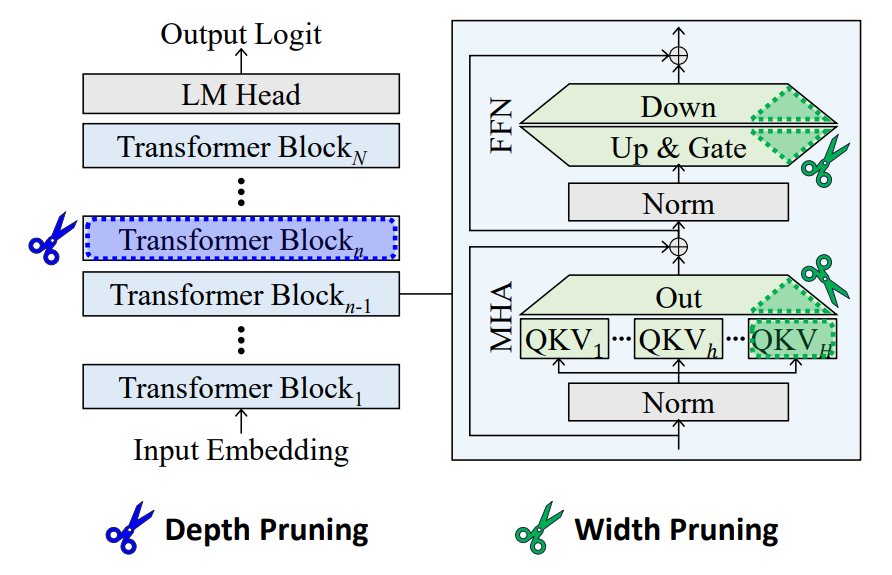
\includegraphics[width=0.7\textwidth]{pruning.png}
    \caption[Comparison of Depth and Width Pruning]{In depth pruning, we remove the single transformer layers (left). On the other hand, in width pruning we remove single neurons from the weight matrices (right). The image was retrieved from \cite{shortened_llama}.}
    \label{fig:pruning_comparison}
\end{figure}

\subsection{Depth Pruning} \label{depth_pruning}

As for depth pruning, the approach used in this project eliminates entire attention blocks following the methodology established by Kim et al. in their Shortened LLaMA work \cite{shortened_llama}, in which they establish four metrics to determine the importance of a transformer block:

\begin{itemize}
   \item \textbf{Magnitude-based importance}: computes L1 norms of weights within each block, assuming that layers with larger weight magnitudes contribute more significantly to model output.
   
   \item \textbf{Taylor expansion importance}: leverages gradient information to estimate removal impact through the approximation 
   \begin{equation}
    L(W = 0) \approx L(W) + \nabla L \cdot (-W)
   \end{equation}
   where the gradient-weight product indicates layer significance based on how loss would change if the layer were removed.
   
   \item \textbf{Perplexity-based importance}: temporarily removes each layer and measures performance degradation on calibration data through perplexity, providing a direct empirical assessment of layer contribution to model quality (details on this metric will be further explained in Section \ref{evaluation}).
\end{itemize}

The implementation employs a combined Taylor-perplexity compound method that merges both gradient-based theoretical estimates and empirical performance measurements. In particular, both the Taylor expansion importance and perplexity-based importance are computed for each layer independently, and the final importance ranking is then determined by averaging the rank positions from both methods. Layers with lower rank scores are considered less important and prioritized for removal.

Following insights from prior work in Section \ref{frankenllama} and Shortened-LLaMA \cite{shortened_llama}, the implementation protects the first four and last two layers from removal, as these positions prove critical for maintaining performance.

The pruning implementation creates a new model architecture with reduced depth by systematically copying weights from the original model while skipping the least important layers. The process begins by modifying the model configuration to reflect the reduced number of layers, then establishes a mapping between original and pruned layer indices. This mapping accounts for the gaps created by removed layers, ensuring that retained layers maintain their relative positioning and connectivity.

The resulting pruned model maintains the same computational pattern as the original but with fewer sequential operations, directly reducing inference latency and, most importantly, memory requirements.

\subsection{Width Pruning} \label{wanda}

The width pruning approach in this pipeline exclusively employs structured pruning techniques to maintain compatibility with modern hardware accelerators while simplifying the compression process. Specifically, the implementation targets structured sparsity patterns supported by NVIDIA's sparse Tensor Cores in Ampere and Hopper architectures \cite{nvidia-width}. This sparsity pattern enables theoretical 2x compute throughput compared to dense matrix multiplication while maintaining efficient memory access and good accuracy recovery potential. In other words, unlike unstructured pruning that creates irregular sparse matrices requiring specialized computation libraries, structured sparsity preserves regular tensor shapes that map directly to accelerator capabilities without additional software overhead. A visual representation of the advantage is shown in Figure \ref{fig:nvidia-width}.

\begin{figure}[htbp]
    \centering
    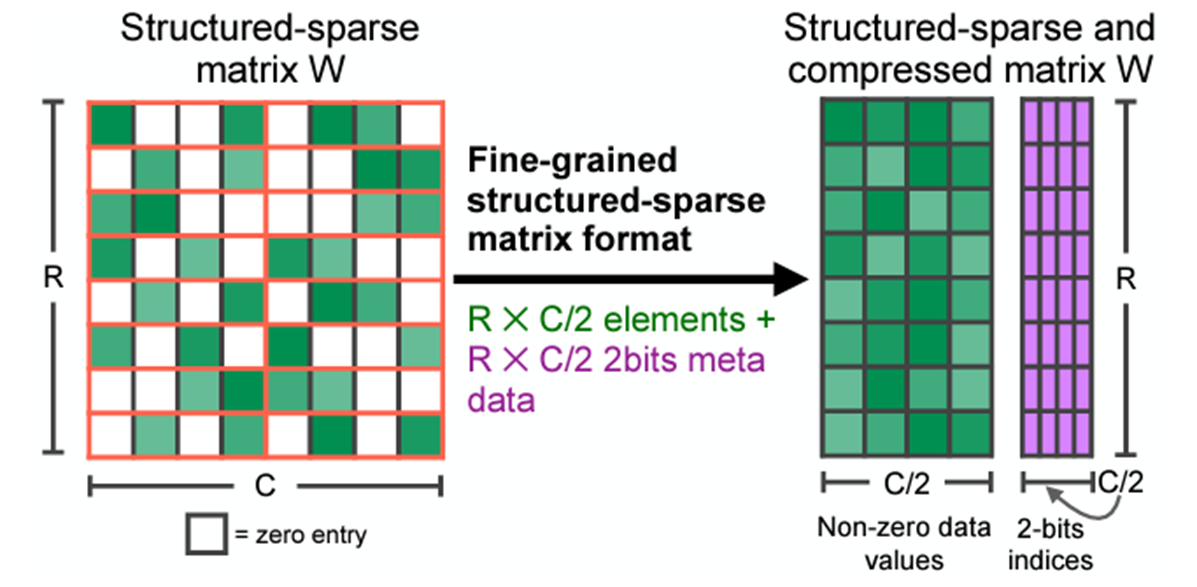
\includegraphics[width=0.7\textwidth]{structured-sparsity-pattern.png}
    \caption[Advantages of Structured Sparsity]{Visual representation of how the structured-sparse matrices are processed in NVIDIA's Ampere and Hopper GPUs. The image was sourced from \cite{nvidia-width}.}
    \label{fig:nvidia-width}
\end{figure}

\textit{Weight And activation-based pruning} (WANDA) \cite{wanda} serves as the core algorithm for implementing this structured approach. Originally developed for unstructured weight removal, WANDA's official implementation includes extensions for structured pruning patterns that align with hardware requirements. The method leverages the observation that large language models develop outlier activations, which are emergent features with magnitudes significantly larger than typical hidden state values yet remain crucial for performance. Consequently, the WANDA importance metric for each weight $W_{ij}$ is defined as

\begin{equation}
S_{ij} = |W_{ij}| \cdot \|X_j\|_2
\end{equation}

where $|W_{ij}|$ represents the absolute weight magnitude and $\|X_j\|_2$ evaluates the L2 norm of the $j$-th input feature across calibration samples. This formulation addresses a key limitation of traditional magnitude-based importance, which is typically used by width pruning approaches, by accounting for input activations, which play an equally important role in determining neuron outputs.

The structured pruning process each layer by organizing weights into groups of $M$ consecutive elements (i.e. consecutive columns of the same row of the weight matrix) and removing the $N$ with lowest importance scores while retaining the rest. To achieve this, forward hooks collect activation statistics during calibration, with each linear layer wrapped to compute the L2 norm of input activations across samples. After computing importance scores for each weight group, the implementation uses PyTorch's scatter operations to efficiently mark low-importance weights for removal. The algorithm completes pruning in a single forward pass using the C4 corpus \cite{c4} as calibration dataset.

\section{Low-Rank Adaptation (LoRA)} \label{lora}

\textit{Low-Rank Adaptation} (LoRA) \cite{lora} represents a parameter-efficient fine-tuning technique that addresses the computational and memory constraints associated with full model retraining. Rather than updating all model parameters during adaptation, LoRA introduces trainable low-rank decomposition matrices that capture the essential changes needed for task-specific performance while keeping the original pre-trained weights frozen. Figure \ref{fig:lora} provides an overview of this process.

\begin{figure}[htbp]
    \centering
    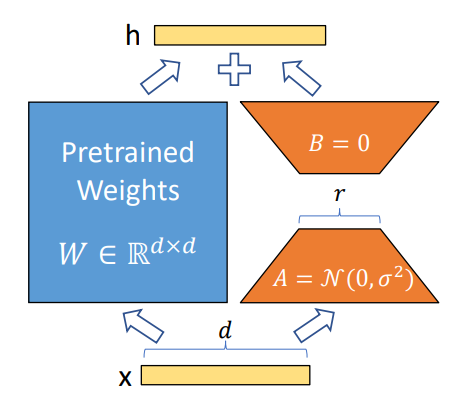
\includegraphics[width=0.4\textwidth]{lora.png}
    \caption[LoRA Overview]{A summary of the LoRA process. We can see how the original pre-trained weights and the low rank adapter are summed when the activation is computed. The image was retrieved from the original LoRA paper \cite{lora}.}
    \label{fig:lora}
\end{figure}

The fundamental insight behind LoRA stems from the hypothesis that weight updates during adaptation have a low intrinsic rank, even when the full rank of the weight matrices is very high. For a pre-trained weight matrix $W_0 \in \mathbb{R}^{d \times k}$, LoRA constrains the update by representing it through a low-rank decomposition:

\begin{equation}
W_0 + \Delta W = W_0 + BA
\end{equation}

where $B \in \mathbb{R}^{d \times r}$, $A \in \mathbb{R}^{r \times k}$, and the rank $r \ll \min(d,k)$. During training, $W_0$ remains frozen while only $A$ and $B$ contain trainable parameters.

The modified forward pass becomes:
\begin{equation}
h = W_0X + \Delta WX = W_0X + BAX
\end{equation}

The matrices are initialized such that $A$ follows a random Gaussian distribution while $B$ is initialized to zero, ensuring that $\Delta W = BA$ starts at zero and the model begins with its original pre-trained behavior. Figure \ref{fig:lora} summarizes the process in a schematic way.

LoRA offers substantial reductions in trainable parameters while maintaining comparable performance to full fine-tuning. Its linear design enables merging the low-rank matrices with frozen weights during deployment, introducing no additional inference latency. According to the original paper, in Transformer architectures, LoRA is most effective when applied to attention weights, particularly the query and value projection matrices ($W_q$ and $W_v$), with very low ranks ($r=1$ or $r=2$) often proving sufficient for downstream tasks.

Within the compression pipeline, LoRA serves as the third stage, following the pruning phases. This positioning is strategic: LoRA helps recover performance degraded by the aggressive structural modifications while simultaneously adapting the model for specific downstream tasks.

The implementation utilizes Hugging Face's \textit{Parameter-Efficient Fine-Tuning} (PEFT) \cite{peft} library, which provides optimized LoRA integration with Hugging Face transformer models. The configuration targets the attention projection matrices with a rank of 8 and dropout rate of 0.1. Training employs mixed-precision optimization with gradient accumulation to maintain computational efficiency while adapting to the reduced parameter space. The calibration process uses 1024 samples from the C4 dataset \cite{c4}.

\section{Quantization} \label{quantization}

Quantization represents a fundamental compression technique that maps continuous floating-point values to a discrete, finite set of representations, typically using low precision formats such as 8-bit or 4-bit integers. This approach is widely used on Large Language Models, as it offers substantial memory reduction with controlled impact on model performance.

The quantization process follows the mapping:
\begin{equation}
q = \text{round}\left(\frac{x - z}{s}\right)
\end{equation}
where $x$ represents the original floating-point value, $s$ denotes the scale factor, $z$ is the zero-point offset, and $q$ is the quantized value. Subtracting the offset and dividing by the scale normalizes the floating-point value to the quantization grid, so that it is accurately represented within the discrete range of the target precision format.

Normally, naive quantization approaches such as round-to-nearest often result in significant accuracy degradation. The GPTQ technique \cite{gptq_quantization} addresses these limitations through a sophisticated post-training quantization algorithm that leverages second-order information to minimize reconstruction error. GPTQ formulates quantization as a layer-wise optimization problem, where for each linear layer with weight matrix $W$ and calibration inputs $X$, the algorithm seeks quantized weights $\hat{W}$ that minimize the reconstruction error:
\begin{equation}
\arg\min_{\hat{W}} ||WX - \hat{W}X||_2^2
\end{equation}

The key innovation enabling scalability to billion-parameter models is the insight that quantizing weights in arbitrary order yields comparable results to greedy selection for large layers, reducing computational complexity from $O(d_{\text{row}} \cdot d_{\text{col}}^3)$ to $O(\max\{d_{\text{row}} \cdot d_{\text{col}}^2, d_{\text{col}}^3\})$. To achieve this efficiency, GPTQ incorporates several practical optimizations: weights are processed in blocks of 128 columns through lazy batch updates, with modifications accumulated and applied globally after each block completion. Additionally, Cholesky decomposition is used to compute Hessian inverse information upfront, ensuring numerical stability for large models. The Hessian matrix is computed as $H = 2XX^T + \lambda I$, where $\lambda$ represents a damping factor for numerical stability.

In our compression pipeline, quantization serves as the fourth stage, applied after pruning and LoRA adaptation phases. This ordering strategically leverages the reduced parameter count from pruning while ensuring the model maintains reasonable performance levels before the additional approximation introduced by quantization. The calibration process utilizes 128 random samples from the training dataset, each containing 2048 tokens, providing sufficient statistical information for accurate quantization while maintaining computational efficiency.

For practical implementation, we employed the GPTQModel PyTorch toolkit \cite{gptqmodel}, which significantly simplifies the quantization process by providing optimized implementations of the GPTQ algorithm with support for various model architectures and quantization configurations. This toolkit handles the complex numerical computations and memory management required for large-scale quantization, allowing focus on the integration aspects within the broader compression pipeline.

For LLaMA 3.2 1B, 4-bit quantization reduces memory requirements from approximately 2GB to 500MB while typically maintaining perplexity increases below 0.5 points on standard language modeling benchmarks. This substantial compression ratio, combined with minimal performance degradation, demonstrates the effectiveness of the GPTQ approach for maintaining model quality while achieving significant memory savings suitable for deployment on resource-constrained hardware.

\subsection{Eigenspace Low-Rank Approximation (EoRA)} \label{eora}

Following quantization, Eigenspace Low-Rank Approximation (EoRA) \cite{eora} can be optionally applied to recover accuracy lost during compression. EoRA is a rather novel technique which provides a training-free method to enhance performance of compressed models through low-rank matrix compensation by projecting compression errors into task-specific eigenspaces. Figure \ref{fig:eora} summarises the process in a schematic way.


\begin{figure}[htbp]
    \centering
    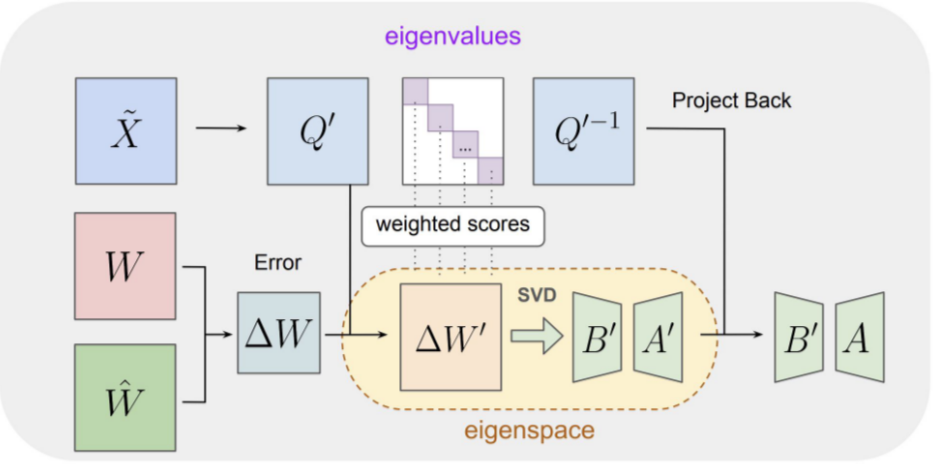
\includegraphics[width=0.7\textwidth]{eora.png}
    \caption[EoRA Representation]{The image summarizes the EoRA process in a schematic way, courtesy of \cite{eora}.}
    \label{fig:eora}
\end{figure}


While their names might be similar, EoRA differs fundamentally from Low-Rank Adaptation (LoRA). While LoRA adapts pre-trained models to new tasks through gradient-based optimization of low-rank matrices, EoRA focuses on compensating compression-induced errors without training. Nevertheless, both methods employ additive low-rank corrections to weight matrices which are formulated as adapters.

As noted earlier, EoRA projects compression error into the eigenspace of layer-wise input activations before applying singular value decomposition. For a layer with original weights $W$ and compressed weights $\hat{W}$, compression error is $\Delta W = W - \hat{W}$. Rather than directly decomposing this error, EoRA first computes the eigendecomposition $\tilde{X}\tilde{X}^T = Q\Lambda Q^T$, where $\tilde{X}$ represents average input activations over the calibration dataset. This is done in order to derive the eigenspace projection matrix $Q$, whose columns are the eigenvectors, and $\Lambda$, which is a diagonal matrix containing the corresponding eigenvalues.

The projection of the compression error into the eigenspace is then computed using the transformation matrix $Q' = Q\sqrt{\Lambda}$:
\begin{equation}
\Delta W' = \Delta W \cdot Q'
\end{equation}

This eigenspace projection amplifies compression errors along directions of high activation variance (i.e. high eigenvalues) while diminishing those along low-variance directions, causing the subsequent SVD to naturally allocate more of its limited representational capacity to approximating the amplified, task-relevant error components.

Finally, the projected error $\Delta W'$ is decomposed using SVD to obtain $\Delta W' \approx B'A'$, where $B'$ and $A'$ are low-rank matrices. The final compensation matrices are obtained by back-projecting to the original space: $A = A'(Q')^{-1}$.

Similarly to LoRA, the forward pass on the compensated model becomes:
\begin{equation}
h = \hat{W}X + B'A'(Q')^{-1}X = \hat{W}X + B'AX
\end{equation}

In the default configuration of the pipeline, the EoRA calibration step uses 64 samples from the C4 dataset \cite{c4}. This minimal calibration requirement is one of the main advantages of this method. Implementation once again leverages the GPTQModel toolkit \cite{gptqmodel}, which integrates EoRA compensation with existing quantized models.


\section{Evaluation} \label{evaluation}
